\documentclass[11pt]{article}

\usepackage[margin=0.75in]{geometry}
\usepackage{array}
\usepackage{booktabs}
\usepackage{graphicx}
\usepackage[table]{xcolor}

\definecolor{boxgreen}{HTML}{DBE6D3}
\definecolor{darkgreen}{HTML}{233423}
\definecolor{midgreen}{HTML}{6D7A63}
\definecolor{lightrow}{HTML}{EEF4EA}

\renewcommand{\arraystretch}{1.18}
\setlength{\parindent}{0pt}
\setlength{\parskip}{6pt}

\title{\textbf{Chapter 18 OOPG Results}\\
\large Catastrophic Payments for Health Care, NLSS IV 2022/23}
\author{Authors' calculations from NLSS IV}
\date{Compiled with MiKTeX \texttt{pdflatex}}

\begin{document}
\pagecolor{boxgreen}
\color{black}
\maketitle

\section*{Scope and Method}

This report follows the Chapter 18 catastrophic-payment framework for
\textbf{OOPG} only. OOPG is the project term for household out-of-pocket
spending on communicable disease or injury from NLSS Section 8(B).

The estimates use household survey weights. The primary denominator convention
is the Wagstaff health-including construction used in the current analysis
pipeline: total expenditure and capacity-to-pay denominators add total real OOP
back to the NLSS health-excluding welfare aggregate.

\section*{Box 18.1-style Results: Incidence and Intensity}

\begin{table}[!htbp]
\centering
\small
\rowcolors{3}{lightrow}{boxgreen}
\begin{tabular}{>{\raggedright\arraybackslash}p{0.38\textwidth}rrrrr}
\toprule
\textbf{Catastrophic payment measure} & \textbf{5\%} & \textbf{10\%} & \textbf{15\%} & \textbf{25\%} & \textbf{40\%} \\
\midrule
\multicolumn{6}{l}{\emph{OOPG as share of total expenditure}} \\
Head count (H) & 13.97\% & 6.72\% & 3.65\% & 1.58\% & 0.70\% \\
standard error & 0.61\% & 0.38\% & 0.26\% & 0.16\% & 0.10\% \\
Overshoot (O) & 1.23\% & 0.75\% & 0.50\% & 0.25\% & 0.09\% \\
standard error & 0.07\% & 0.06\% & 0.04\% & 0.03\% & 0.02\% \\
Mean positive overshoot (MPO) & 8.81\% & 11.14\% & 13.73\% & 16.12\% & 13.29\% \\
\addlinespace
\multicolumn{6}{l}{\emph{As share of capacity-to-pay expenditure}} \\
Head count (H) & --- & --- & 9.08\% & 4.52\% & 1.96\% \\
standard error & --- & --- & 0.46\% & 0.31\% & 0.18\% \\
Overshoot (O) & --- & --- & 1.42\% & 0.78\% & 0.33\% \\
standard error & --- & --- & 0.09\% & 0.06\% & 0.04\% \\
Mean positive overshoot (MPO) & --- & --- & 15.68\% & 17.31\% & 16.80\% \\
\bottomrule
\end{tabular}
\caption{Incidence and intensity of catastrophic OOPG payments, Nepal NLSS IV 2022/23.}
\end{table}

\section*{Book-style Figure}

\begin{figure}[!htbp]
\centering
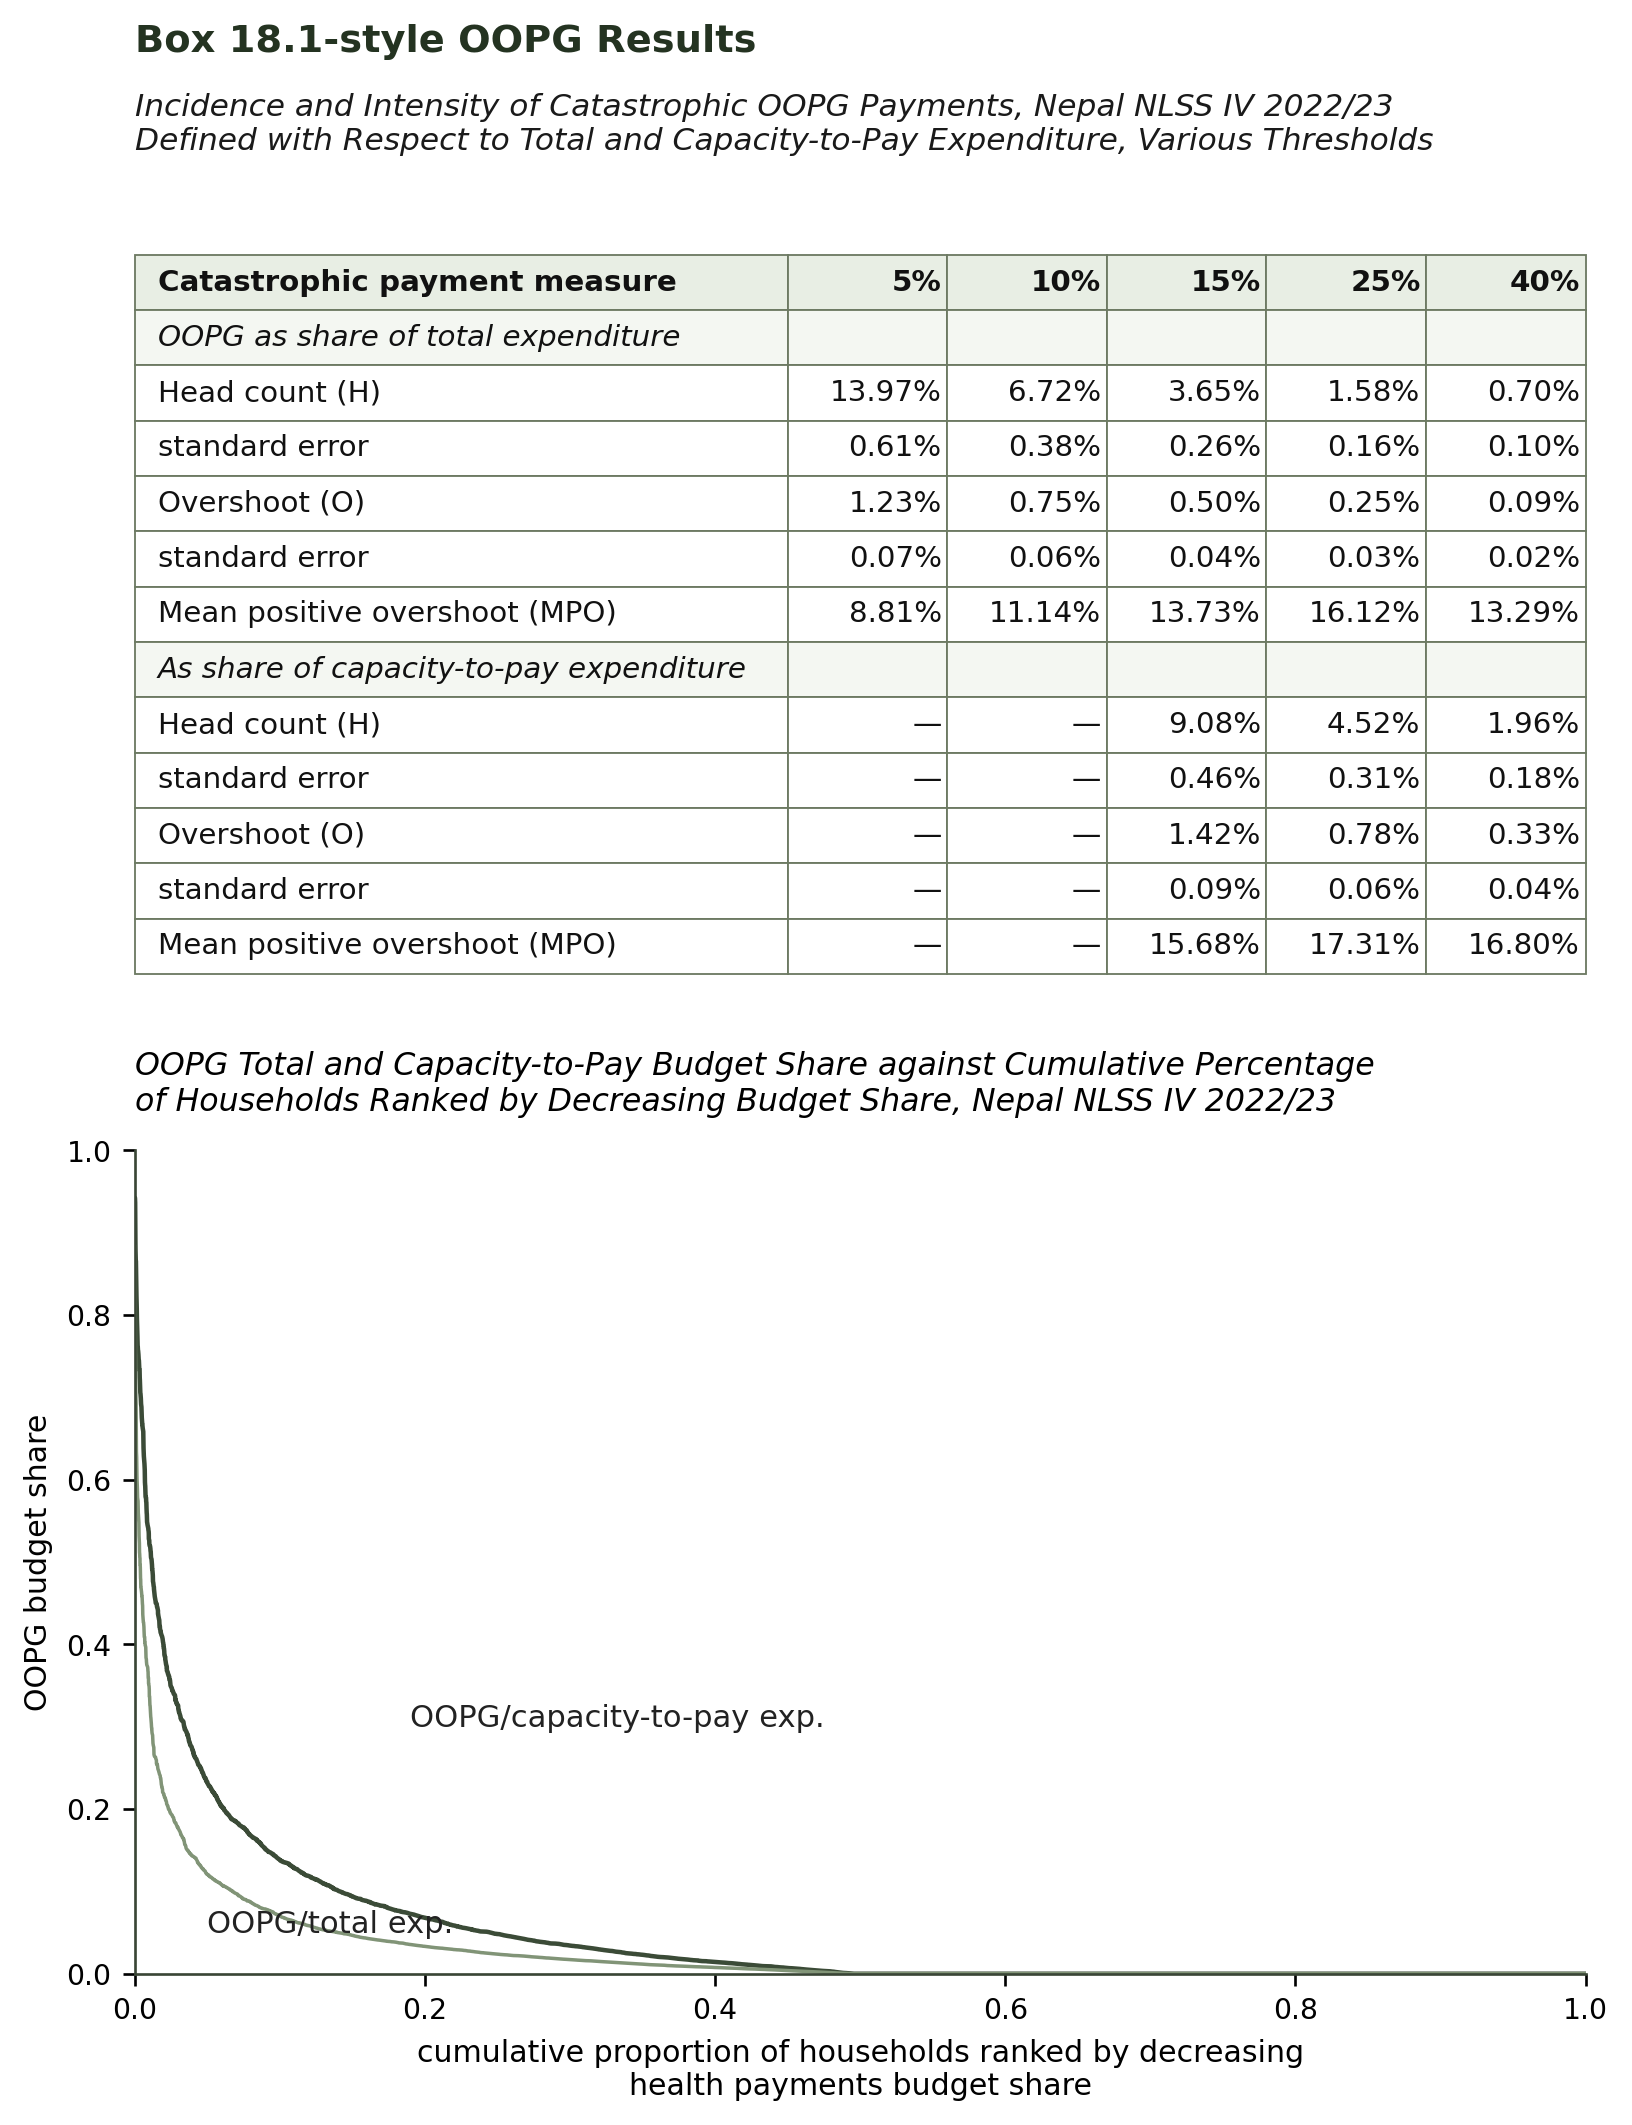
\includegraphics[width=0.86\textwidth,height=0.78\textheight,keepaspectratio]{oopg_box18_1_incidence_intensity.png}
\caption{Book-style table and budget-share curve for OOPG.}
\end{figure}

\clearpage

\section*{Box 18.2-style Results: Distribution-Sensitive Measures}

\begin{table}[!htbp]
\centering
\small
\rowcolors{3}{lightrow}{boxgreen}
\begin{tabular}{>{\raggedright\arraybackslash}p{0.42\textwidth}rrrrr}
\toprule
\textbf{Distribution-sensitive measure} & \textbf{5\%} & \textbf{10\%} & \textbf{15\%} & \textbf{25\%} & \textbf{40\%} \\
\midrule
\multicolumn{6}{l}{\emph{OOPG as share of total expenditure}} \\
Concentration index, $C^{H}$ & -0.0053 & 0.0740 & 0.1517 & 0.3308 & 0.5004 \\
Rank-weighted head count, $H^{W}$ & 14.04\% & 6.22\% & 3.09\% & 1.05\% & 0.35\% \\
Concentration index, $C^{O}$ & 0.1846 & 0.2902 & 0.3808 & 0.5317 & 0.6585 \\
Rank-weighted overshoot, $O^{W}$ & 1.00\% & 0.53\% & 0.31\% & 0.12\% & 0.03\% \\
\addlinespace
\multicolumn{6}{l}{\emph{As share of capacity-to-pay expenditure}} \\
Concentration index, $C^{H}$ & --- & --- & -0.0255 & 0.0602 & 0.1865 \\
Rank-weighted head count, $H^{W}$ & --- & --- & 9.32\% & 4.25\% & 1.60\% \\
Concentration index, $C^{O}$ & --- & --- & 0.1352 & 0.2336 & 0.3885 \\
Rank-weighted overshoot, $O^{W}$ & --- & --- & 1.23\% & 0.60\% & 0.20\% \\
\bottomrule
\end{tabular}
\caption{Distribution-sensitive catastrophic OOPG payment measures. Households are ranked by pre-OOP welfare.}
\end{table}

\begin{figure}[!htbp]
\centering
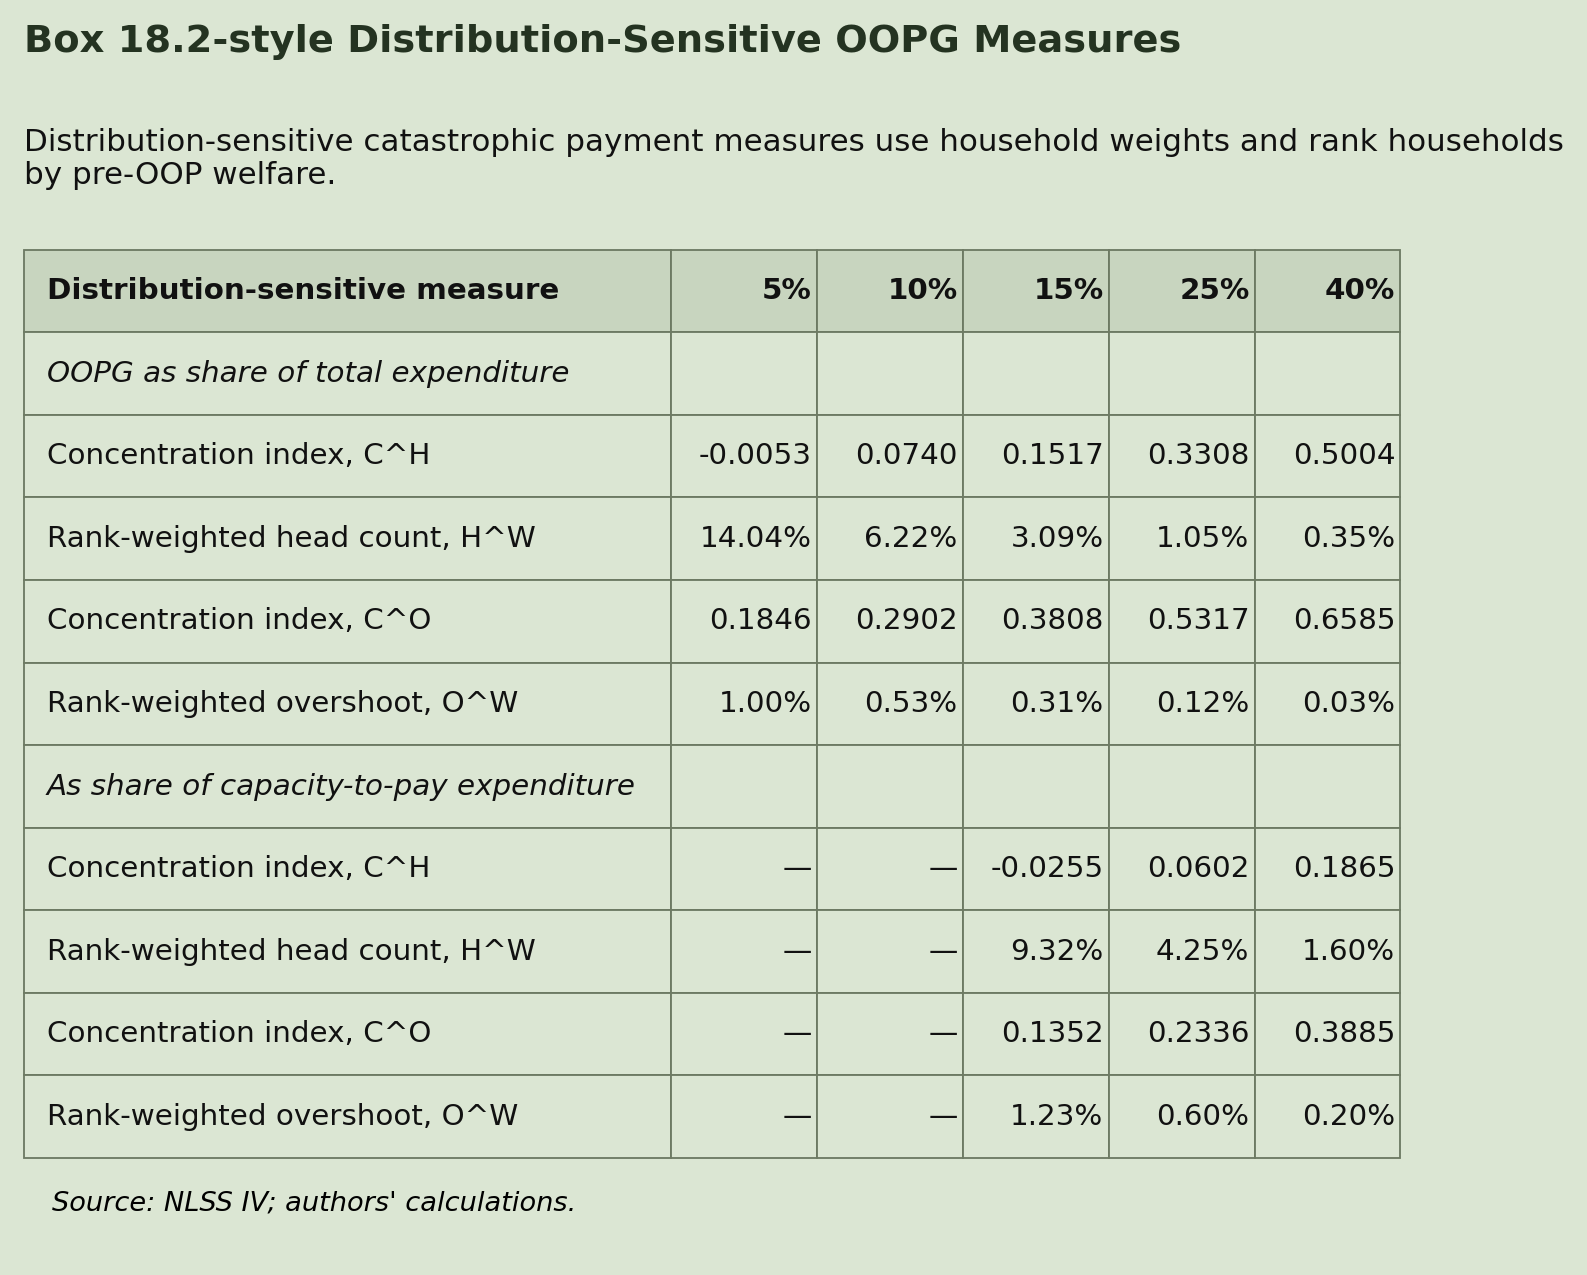
\includegraphics[width=0.92\textwidth,height=0.74\textheight,keepaspectratio]{oopg_box18_2_distribution_sensitive.png}
\caption{Book-style distribution-sensitive OOPG output.}
\end{figure}

\section*{Short Interpretation}

At the 10\% total-expenditure threshold, 6.72\% of households experience
catastrophic OOPG payments. The corresponding overshoot is 0.75\%, meaning
that, averaged over all households, OOPG payments exceed the 10\% threshold by
0.75 percentage points. Among households that cross the threshold, the mean
positive overshoot is 11.14\%.

Using the capacity-to-pay denominator, the 40\% threshold identifies 1.96\% of
households as catastrophic. The concentration index for this headcount is
0.1865, while the rank-weighted headcount is 1.60\%. These results suggest that
the OOPG catastrophic burden is present but relatively concentrated in a smaller
set of households.

\end{document}
